% This file allows to produce either a separate PDF/PNG image
% See standalone documentation to understand underlying magic

\documentclass[tikz,convert={density=150,size=600,outext=.png}]{standalone}
\usetikzlibrary{shapes, calc, arrows, fit, positioning, decorations, patterns, decorations.pathreplacing, chains, snakes}
\input{../setup-web-fonts}
\input{../setup-packages}
\graphicspath{{../pictures/}} % path to pictures, trailing slash is mandatory.

% The actual drawing follows
\begin{document}
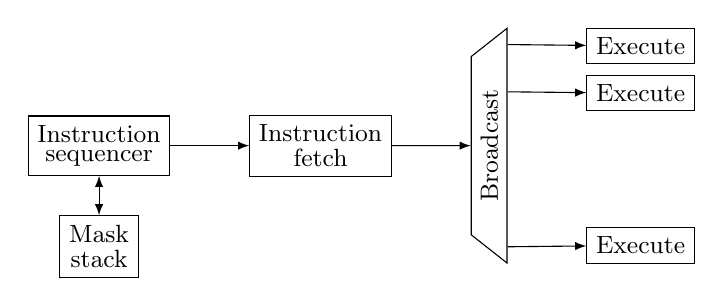
\begin{tikzpicture}[>=latex, font=\small]

\node[draw, rectangle] (sequencer) {\shortstack{Instruction\\sequencer}};
\node[draw, rectangle, below=0.5cm of sequencer] (stack) {\shortstack{Mask\\stack}};
\node[draw, rectangle, right=1cm of sequencer] (fetch) {\shortstack{Instruction\\fetch}};
\node[draw, trapezium, trapezium stretches, right=1cm of fetch, rotate=90, anchor=north, minimum width=3cm] (broadcast) {Broadcast};
\node[draw, rectangle, above right=0.8cm and 1cm of broadcast.south east] (exec1) {Execute};
\node[draw, rectangle, above right=0.2cm and 1cm of broadcast.south east] (exec2) {Execute};
\node[draw, rectangle, below right=0.8cm and 1cm of broadcast.south west] (execN) {Execute};

\draw[<->] (sequencer) -- (stack);
\draw[->] (sequencer) -- (fetch);
\draw[->] (fetch) -- (broadcast);
\draw[->] ([yshift=1.05cm] broadcast.south east) -- (exec1);
\draw[->] ([yshift=0.45cm] broadcast.south east) -- (exec2);
\draw[->] ([yshift=-1.05cm] broadcast.south west) -- (execN);

\end{tikzpicture}

\end{document}
